\documentclass[conference]{IEEEtran}
\usepackage{cite}
\usepackage{amsmath,amssymb,amsfonts}
\usepackage{graphicx}
\usepackage{textcomp}
\usepackage{xcolor}
\usepackage{multicol}
\usepackage{float}
\usepackage[spanish]{babel}
\usepackage[spanish,vlined,ruled,]{algorithm2e}

\def\BibTeX{{\rm B\kern-.05em{\sc i\kern-.025em b}\kern-.08em
    T\kern-.1667em\lower.7ex\hbox{E}\kern-.125emX}}
\begin{document}

\title{Morphing}
\author{\IEEEauthorblockN{Joaquín Pérez Araya}
\IEEEauthorblockA{\textit{Departamento de Ciencias de la Computación} \\
\textit{Universidad de Chile}\\
Santiago, Chile \\
joaquin.perez.a@ug.uchile.cl}}


\maketitle

\begin{abstract}
	
\end{abstract}
 

\section*{Introducción} % ***Así la cosa no me molesta con los numeritos***
	El \textit{morphing} un tipo de efecto visual el cual se produce al cambiar una imagen a otra con un efecto de metamorfosis, actualmente se utiliza principalmente para el entretenimiento. En este documento se implementará el algoritmo descrito por Beier-Neely\cite{Paper}, que consiste en utilizar líneas de correspondencia entre la imagen de partida y la imagen de destino para describir la forma en que la mutación se va a llevar a cabo. Primero se describirá el diseño en la implementación
	
	
\section*{Diseño e Implementación}
	El código implementado se define en 3 funciones las cuales están implementadas en \texttt{morphing.py}: \textit{warp}, \textit{morph} y \textit{create morphing video}: La transformación de una imagen según un par de conjuntos de líneas (\textit{warp}), la creación de múltiples imágenes que son las que forman parte del morphing (\textit{morph}) y finalmente la creación, a partir de las imágenes calculadas en el proceso anterior el vídeo que muestra el cambio de las imágenes a lo largo del tiempo \textit{create morphing video}. También se dispone de un módulo adicional llamado \texttt{util.py} el cual contiene funciones auxiliares.
	
	\subsection*{Warpping}
		Para el warpping se utiliza el algoritmo propuesto en el artículo\cite{Paper}, que está especificado en el Algoritmo 1, el cual crea una imagen vacía con las mismas dimensiones de la imagen fuente, y itera sobre ésta, calculando qué colores debería tener según las líneas de correspondencia y la imagen fuente.

	\begin{algorithm}[ht]
		\caption{Warpping}	
		\KwData{$image$ imagen fuente, $lines_{src}$ líneas fuente, $lines_{dst}$ líneas de destino.}
		\KwResult{Imagen que corresponde a la imagen fuente modificada según las líneas dadas.}
		\DontPrintSemicolon
	$destinationImage = zeros(shape(image)) $ \;
	\For{Pixel $X$ in $image$}{
		$DSUM = (0,0)$ \;
		$weightsum = 0$ \;
	\For{Line $P_i Q_i$ in $lines_{src}$ and $ P_i^{\prime} Q_i^{\prime}$ in $lines_{dst}$}{
	$u, v = calculate\_u\_v(X,P_i, Q_i)$ \;
	$X^\prime = calculate\_X^\prime (u,v,P_i^{\prime}, Q_i^{\prime})$ \;
	$D_i = X_i^\prime - X$		\;
	$weight = calculate\_weight(X, u, v, P_i, Q_i)$ \;
	$DSUM += D_i * weight$ \;
	$weightsum += weight$ \;
			}		
	$\bar{X} = X + DSUM / weightsum$
	$destinationImage(X) = image(\bar{X})$ \;		
		}
		\KwRet{$destinationImage$}
		\label{asdf}
		\end{algorithm} 

		Para los parámetros del peso se eligió: $A = 1, B = 1, p= 0.5$
		En el módulo de utilidades, están implementadas las funciones para el cálculo de $u$, $v$, $X^\prime$ y $weight$ según como se indica en el artículo.
	
	La implementación usa el algoritmo en su versión \textit{inverse mapping}, es decir durante la ejecución se recorre la imagen de destino calculando qué pixeles de la imagen original deberían estar allí utilizando interpolación bilineal de los pixeles más cercanos de la imagen original, este método ofrece más simplicidad dado que se conoce los pixeles de destino de antemano por lo que el único inconveniente es el caso de que se requieren píxeles fuera de la imagen original por lo que se interpola según los pixeles ya calculados anteriormente, en cuyo caso sería:
		\begin{itemize}
               	\item Si se está en el primer pixel de la imagen, el de la esquina superior izquierda, éste se calcula como el pixel del mismo punto de la imagen de origen.
               	\item Si se está en la fila superior, se calcula usando el pixel anterior calculado, el de la izquierda de éste.
               	\item Si se está en la columna de la izquierda, se calcula usando el pixel de la fila superior.
               	\item Si se está en la columna de la derecha, se calcula utilizando los 3 pixeles que están cercanos a éste: Superior izquierdo, superior e izquierdo.
               	\item De otra forma se calcula utilizando 4 pixeles cercanos: Superior izquierdo, superior, superior derecho e izquierdo.
		\end{itemize}
	
	\subsection*{Morphing y Video}
	Para la creación del conjunto de imágenes que forman el Morphing completo se realiza lo siguiente: se itera por el número de imágenes $n$ que uno quiere incluir en el vídeo, se calcula el valor de entrelazado $t$ que va desde $0$ hasta $1$ de $\frac{1}{n}$ en $\frac{1}{n}$ pasos, según el grado de avance del Morphing. \\
	Dado un $t$ de éste proceso, para crear una imagen, se realiza un cross-fade entre dos imágenes: el \textit{warp} de la imagen fuente con sus líneas y la interpolación de las líneas fuente hacia las líneas de destino según $t$, es decir $t \cdot lines_{src} + (1 - t) \cdot lines_{dst}$, y el \textit{warp} entre la imagen de destino con sus líneas y la interpolación de las líneas de destino hacia las fuentes según $t$, que es $(1 - t) \cdot lines_{src} + t \cdot lines_{dst}$. Al final se añade a la colección de imágenes la ponderación de $t$ por la primera imagen más $1 - t$ de la segunda. \\
	
	Luego de finalizado la creación de la colección de imágenes del morphing, se utiliza la librería de OPENCV para formar un vídeo con éstas, en esta implementación, los vídeos generados están a 10 cuadros por segundo y en formato \texttt{.avi}.


\section*{Experimentación}
	Se realizaron pruebas con dos pares de imágenes: Una con un par con dos felinos distinos, un puma y una leona, y la otra con un par de dos actores famosos. Para prueba se crearon 3 conjuntos de líneas, uno con líneas de contorno (véase las líneas verdes en la figura 1), uno con líneas de expresión (las líneas azules en la misma figura) y por último uno con ambas líneas en conjunto.
	
\begin{figure}[H]
\begin{multicols}{2}
    \centering
    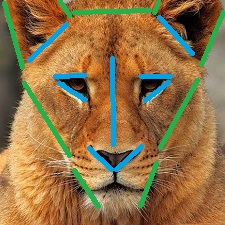
\includegraphics[width=0.98\linewidth]{cats/cat1 lines.jpg} \par
    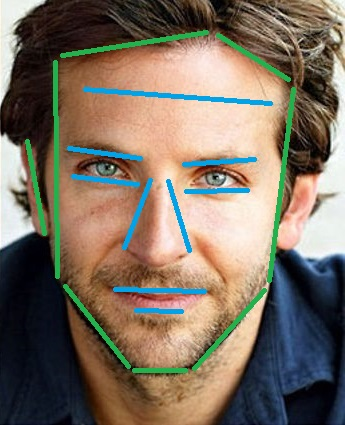
\includegraphics[width=0.98\linewidth]{faces/face1 lines.jpg} \par
    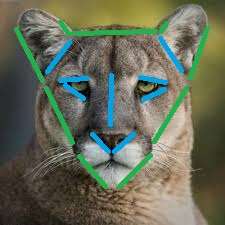
\includegraphics[width=0.98\linewidth]{cats/cat2 lines.jpg} \par
    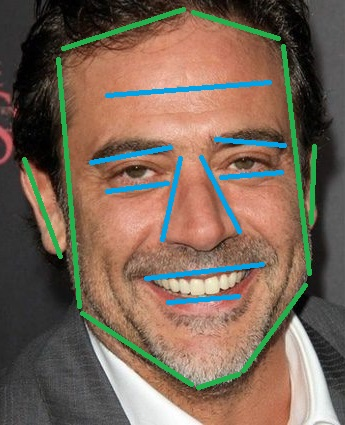
\includegraphics[width=0.98\linewidth]{faces/face2 lines.jpg} \par
\end{multicols}
\caption{Imágenes usadas para la experimentación, están marcadas las líneas utilizadas para el Morphing, las verdes corresponden a contornos de la figura mientras que las azules corresponden a características intrínsecas de la imagen. Las imágenes de la izquierda corresponden a las de fuente mientras que las de la derecha corresponden a las de destino.}
\end{figure}
	
	Para cada prueba, se ejecutó la implementación requiriendo 50 imágenes en total, de las cuales, por motivos de simplicidad, sólo se presentarán la $1^{ra}, 10^{ma}, 20^{va}, 30^{va}, 40^{va}$ y $50^{va}$ imagen de dichas ejecuciones, sin embargo dentro del directorio de la implementación estarán las pruebas con sus respectivas imágenes y vídeos.
	De aquí en adelante, se mencionará como imágenes verdes, las imágenes que fueron creadas a partir del conjunto de líneas verdes, e imágenes azules de forma análoga. 
	
	\subsection*{Imágenes de Felinos}
\begin{figure}[H]
\begin{multicols}{3}
    \centering
    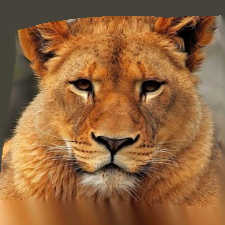
\includegraphics[width=1.0\linewidth]{TestsCats/G/img01.png} \par
    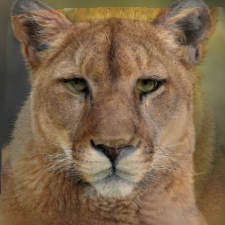
\includegraphics[width=1.0\linewidth]{TestsCats/G/img30.png} \par
    
    \includegraphics[width=1.0\linewidth]{TestsCats/G/img10.png} \par
    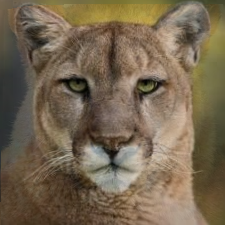
\includegraphics[width=1.0\linewidth]{TestsCats/G/img40.png} \par

    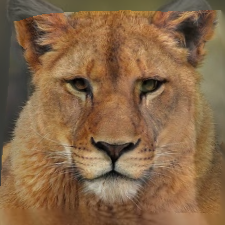
\includegraphics[width=1.0\linewidth]{TestsCats/G/img20.png} \par
    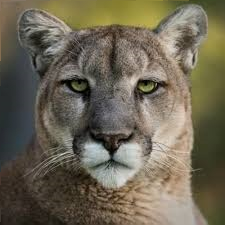
\includegraphics[width=1.0\linewidth]{TestsCats/G/img50.png} \par
\end{multicols}
\caption{Imágenes creadas con la implementación usando sólo las líneas verdes. El progreso va de izquierda a derecha de arriba hacia abajo.}
\end{figure}

\begin{figure}[H]
\begin{multicols}{3}
    \centering
    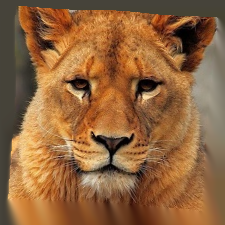
\includegraphics[width=1.0\linewidth]{TestsCats/B/img01.png} \par
    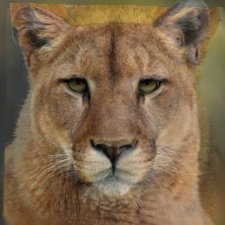
\includegraphics[width=1.0\linewidth]{TestsCats/B/img30.png} \par
    
    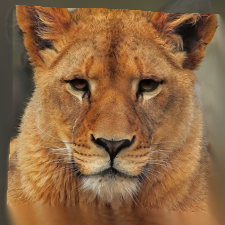
\includegraphics[width=1.0\linewidth]{TestsCats/B/img10.png} \par
    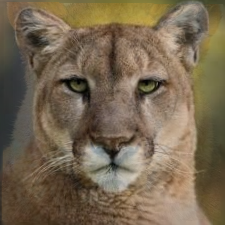
\includegraphics[width=1.0\linewidth]{TestsCats/B/img40.png} \par

    \includegraphics[width=1.0\linewidth]{TestsCats/B/img20.png} \par
    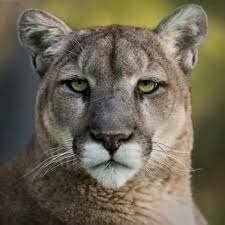
\includegraphics[width=1.0\linewidth]{TestsCats/B/img50.png} \par
\end{multicols}
\caption{Imágenes creadas con la implementación usando sólo las líneas azules. El progreso va de izquierda a derecha de arriba hacia abajo.}
\end{figure}

\begin{figure}[H]
\begin{multicols}{3}
    \centering
    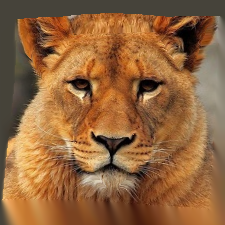
\includegraphics[width=1.0\linewidth]{TestsCats/XL/img01.png} \par
    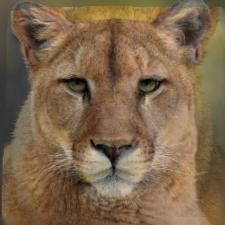
\includegraphics[width=1.0\linewidth]{TestsCats/XL/img30.png} \par
    
    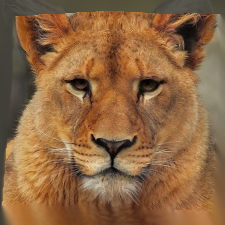
\includegraphics[width=1.0\linewidth]{TestsCats/XL/img10.png} \par
    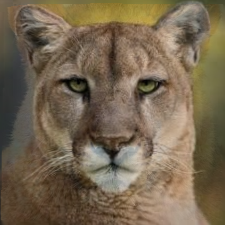
\includegraphics[width=1.0\linewidth]{TestsCats/XL/img40.png} \par

    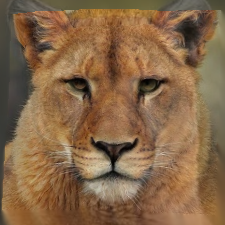
\includegraphics[width=1.0\linewidth]{TestsCats/XL/img20.png} \par
    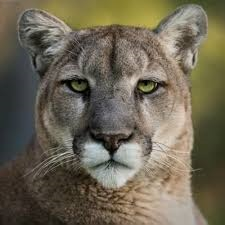
\includegraphics[width=1.0\linewidth]{TestsCats/XL/img50.png} \par
\end{multicols}
\caption{Imágenes creadas con la implementación usando todas las líneas. El progreso va de izquierda a derecha de arriba hacia abajo.}
\end{figure}
	
	Con el conjunto de imágenes obtenidas con los diferentes experimentos se observa que en las imágenes creadas usando las líneas verdes (de contorno), la imagen inicial se dobla para hacer calzar las orejas de ambos felinos, creando así una aparcición de las orejas más armoniosa que en el caso de las imágenes creadas utilizando sólo las líneas azules, sin embargo, el conjunto de imágenes verdes presenta discordancias con las facciones de la cara de los felinos, éstas son más aparentes en la cuarta imagen (la primera de la segunda fila), donde se evidencian éstas en ojos y en nariz. Estos dos detalles no están presentes en las imágenes que usan todas las líneas.


	\subsection*{Imágenes de Caras}
\begin{figure}[H]
\begin{multicols}{3}
    \centering
    \includegraphics[width=1.0\linewidth]{TestsFaces/G/img01.png} \par
    \includegraphics[width=1.0\linewidth]{TestsFaces/G/img30.png} \par
    
    \includegraphics[width=1.0\linewidth]{TestsFaces/G/img10.png} \par
    \includegraphics[width=1.0\linewidth]{TestsFaces/G/img40.png} \par

    \includegraphics[width=1.0\linewidth]{TestsFaces/G/img20.png} \par
    \includegraphics[width=1.0\linewidth]{TestsFaces/G/img50.png} \par
\end{multicols}
\caption{Imágenes creadas con la implementación y con ambos pares de líneas. El progreso va de izquierda a derecha de arriba hacia abajo.}
\end{figure}


\begin{figure}[H]
\begin{multicols}{3}
    \centering
    \includegraphics[width=1.0\linewidth]{TestsFaces/B/img01.png} \par
    \includegraphics[width=1.0\linewidth]{TestsFaces/B/img30.png} \par
    
    \includegraphics[width=1.0\linewidth]{TestsFaces/B/img10.png} \par
    \includegraphics[width=1.0\linewidth]{TestsFaces/B/img40.png} \par

    \includegraphics[width=1.0\linewidth]{TestsFaces/B/img20.png} \par
    \includegraphics[width=1.0\linewidth]{TestsFaces/B/img50.png} \par
\end{multicols}
\caption{Imágenes creadas con la implementación y con ambos pares de líneas. El progreso va de izquierda a derecha de arriba hacia abajo.}
\end{figure}

\begin{figure}[H]
\begin{multicols}{3}
    \centering
    \includegraphics[width=1.0\linewidth]{TestsFaces/XL/img01.png} \par
    \includegraphics[width=1.0\linewidth]{TestsFaces/XL/img30.png} \par
    
    \includegraphics[width=1.0\linewidth]{TestsFaces/XL/img10.png} \par
    \includegraphics[width=1.0\linewidth]{TestsFaces/XL/img40.png} \par

    \includegraphics[width=1.0\linewidth]{TestsFaces/XL/img20.png} \par
    \includegraphics[width=1.0\linewidth]{TestsFaces/XL/img50.png} \par
\end{multicols}
\caption{Imágenes creadas con la implementación y con ambos pares de líneas. El progreso va de izquierda a derecha de arriba hacia abajo.}
\end{figure}

\section*{Conclusión}
	El uso de líneas de contorno (verdes) y líneas de características internas (azules) permiten obtener un \textit{morphing} con pocos errores de discordancias, sin embargo, resulta aún más efectivo combinar ambos tipos de líneas. Desafortunadamente esta técnica se vuelve mucho más lenta con cada línea adicional que se agrega, dado que se deben realizar una iteración de \textit{warping} más para obtener la contribución de ésta línea a los puntos de la imagen de destino, por lo que agregar tanto como líneas de contorno como líneas de características internas tendrán un costo importante en el tiempo de ejecución. De esta forma se tiene que priorizar qué líneas se deben incluir si se está buscando el balance entre errores y tiempo de ejecución.
		
	
\begin{thebibliography}{99}
	 \bibitem{Paper} T. Bier, S. Neely. Feature-Based Image Metamorphosis, Computer Graphics 1992-07

\end{thebibliography}

\end{document}

\begin{figure}[H]
    \centering
    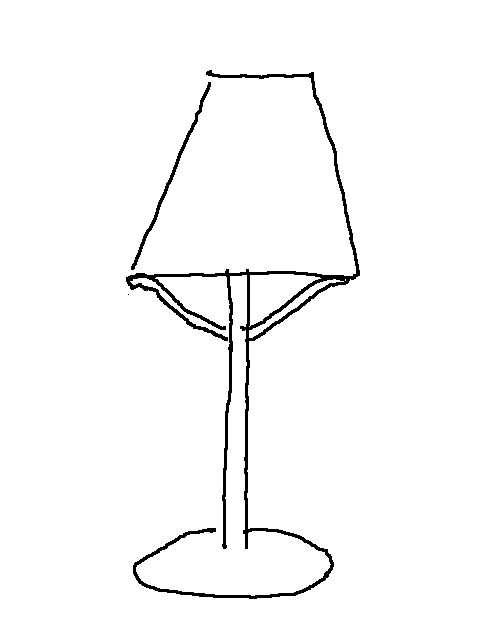
\includegraphics[width=0.95\linewidth]{image/lamps.jpg} \par

\caption{Ejemplo de una posible búsqueda, la imagen de la izquierda representa el dibujo de búsqueda y las de la derecha los resultados esperados.}
\end{figure}